\documentclass{standalone}
\usepackage{tikz}
\usepackage{xcolor}
\usetikzlibrary{patterns, positioning}
\usetikzlibrary{shapes.misc}
\usepackage[outline]{contour}
\contourlength{1.5pt} 


\begin{document}
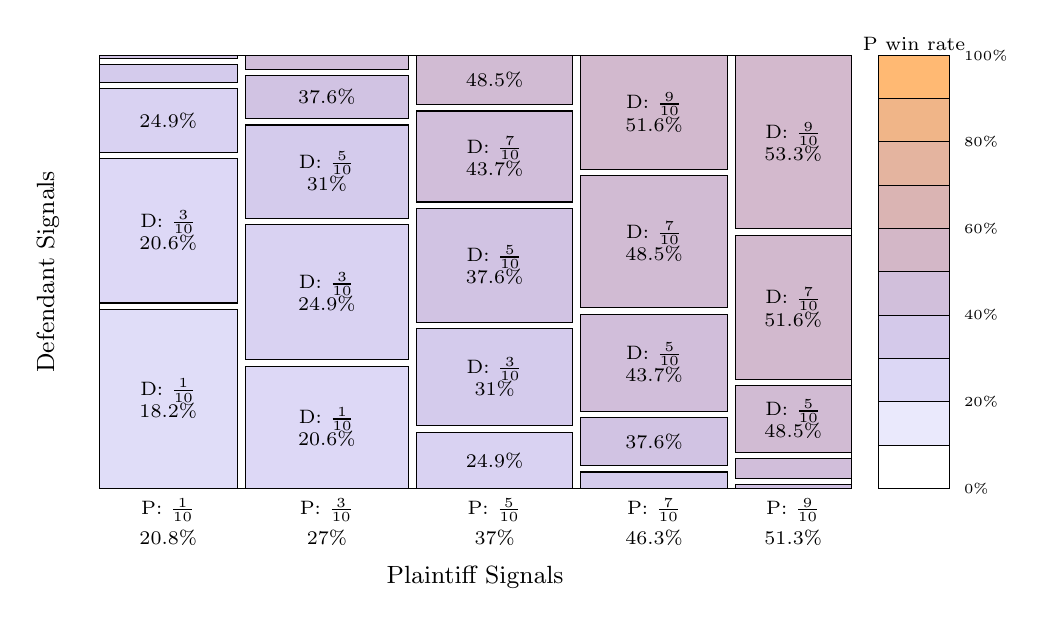
\begin{tikzpicture}
\newcommand{\DFractionOffset}{0.4}
\newcommand{\AxisLabelYAdjust}{-0.235}
\draw[draw=black] (0.6,2) rectangle (10.15,7.5);
\draw[fill=blue!82!orange!18!white!82!white, draw=black] (0.6,2) rectangle (2.3549,4.2748);
\draw (1.477427834898296, 3.137384052801007) node[font=\scriptsize, text=black, align=center] {D: $\frac{1}{10}$\\ 18.2\%};
\draw[fill=blue!79!orange!21!white!81!white, draw=black] (0.6,4.3548) rectangle (2.3549,6.1906);
\draw (1.477427834898296, 5.272664183087704) node[font=\scriptsize, text=black, align=center] {D: $\frac{3}{10}$\\ 20.6\%};
\draw[fill=blue!75!orange!25!white!80!white, draw=black] (0.6,6.2706) rectangle (2.3549,7.0782);
\draw (1.477427834898296, 6.674380087285738) node[font=\scriptsize, text=black, align=center] {24.9\%};
\draw[fill=blue!69!orange!31!white!78!white, draw=black] (0.6,7.1582) rectangle (2.3549,7.3794);
\draw[fill=blue!62!orange!38!white!76!white, draw=black] (0.6,7.4594) rectangle (2.3549,7.5);
\draw (1.477427834898296, 1.6) node[anchor=north, font=\scriptsize, text=black] {20.8\%};
\draw (1.477427834898296, {1.6 + \DFractionOffset}) node[anchor=north, font=\scriptsize, text=black] {P: $\frac{1}{10}$};
\draw[fill=blue!79!orange!21!white!81!white, draw=black] (2.4549,2) rectangle (4.5297,3.5527);
\draw (3.492290943274269, 2.7763256065413096) node[font=\scriptsize, text=black, align=center] {D: $\frac{1}{10}$\\ 20.6\%};
\draw[fill=blue!75!orange!25!white!80!white, draw=black] (2.4549,3.6327) rectangle (4.5297,5.3501);
\draw (3.492290943274269, 4.491379944148136) node[font=\scriptsize, text=black, align=center] {D: $\frac{3}{10}$\\ 24.9\%};
\draw[fill=blue!69!orange!31!white!78!white, draw=black] (2.4549,5.4301) rectangle (4.5297,6.615);
\draw (3.492290943274269, 6.022539010048925) node[font=\scriptsize, text=black, align=center] {D: $\frac{5}{10}$\\ 31\%};
\draw[fill=blue!62!orange!38!white!76!white, draw=black] (2.4549,6.695) rectangle (4.5297,7.2452);
\draw (3.492290943274269, 6.970079202132694) node[font=\scriptsize, text=black, align=center] {37.6\%};
\draw[fill=blue!56!orange!44!white!74!white, draw=black] (2.4549,7.3252) rectangle (4.5297,7.5);
\draw (3.492290943274269, 1.6) node[anchor=north, font=\scriptsize, text=black] {27\%};
\draw (3.492290943274269, {1.6 + \DFractionOffset}) node[anchor=north, font=\scriptsize, text=black] {P: $\frac{3}{10}$};
\draw[fill=blue!75!orange!25!white!80!white, draw=black] (4.6297,2) rectangle (6.616,2.7135);
\draw (5.622859449139195, 2.356772630988808) node[font=\scriptsize, text=black, align=center] {24.9\%};
\draw[fill=blue!69!orange!31!white!78!white, draw=black] (4.6297,2.7935) rectangle (6.616,4.0313);
\draw (5.622859449139195, 3.412402940276162) node[font=\scriptsize, text=black, align=center] {D: $\frac{3}{10}$\\ 31\%};
\draw[fill=blue!62!orange!38!white!76!white, draw=black] (4.6297,4.1113) rectangle (6.616,5.5567);
\draw (5.622859449139195, 4.8339933373271) node[font=\scriptsize, text=black, align=center] {D: $\frac{5}{10}$\\ 37.6\%};
\draw[fill=blue!56!orange!44!white!74!white, draw=black] (4.6297,5.6367) rectangle (6.616,6.7934);
\draw (5.622859449139195, 6.215086959677489) node[font=\scriptsize, text=black, align=center] {D: $\frac{7}{10}$\\ 43.7\%};
\draw[fill=blue!51!orange!49!white!72!white, draw=black] (4.6297,6.8734) rectangle (6.616,7.5);
\draw (5.622859449139195, 7.186723931637742) node[font=\scriptsize, text=black, align=center] {48.5\%};
\draw (5.622859449139195, 1.6) node[anchor=north, font=\scriptsize, text=black] {37\%};
\draw (5.622859449139195, {1.6 + \DFractionOffset}) node[anchor=north, font=\scriptsize, text=black] {P: $\frac{5}{10}$};
\draw[fill=blue!69!orange!31!white!78!white, draw=black] (6.716,2) rectangle (8.5795,2.2083);
\draw[fill=blue!62!orange!38!white!76!white, draw=black] (6.716,2.2883) rectangle (8.5795,2.9009);
\draw (7.647734213885039, 2.594576923107754) node[font=\scriptsize, text=black, align=center] {37.6\%};
\draw[fill=blue!56!orange!44!white!74!white, draw=black] (6.716,2.9809) rectangle (8.5795,4.2138);
\draw (7.647734213885039, 3.597362989637606) node[font=\scriptsize, text=black, align=center] {D: $\frac{5}{10}$\\ 43.7\%};
\draw[fill=blue!51!orange!49!white!72!white, draw=black] (6.716,4.2938) rectangle (8.5795,5.973);
\draw (7.647734213885039, 5.13340184837396) node[font=\scriptsize, text=black, align=center] {D: $\frac{7}{10}$\\ 48.5\%};
\draw[fill=blue!48!orange!52!white!71!white, draw=black] (6.716,6.053) rectangle (8.5795,7.5);
\draw (7.647734213885039, 6.776486034418021) node[font=\scriptsize, text=black, align=center] {D: $\frac{9}{10}$\\ 51.6\%};
\draw (7.647734213885039, 1.6) node[anchor=north, font=\scriptsize, text=black] {46.3\%};
\draw (7.647734213885039, {1.6 + \DFractionOffset}) node[anchor=north, font=\scriptsize, text=black] {P: $\frac{7}{10}$};
\draw[fill=blue!62!orange!38!white!76!white, draw=black] (8.6795,2) rectangle (10.15,2.0485);
\draw[fill=blue!56!orange!44!white!74!white, draw=black] (8.6795,2.1285) rectangle (10.15,2.3752);
\draw[fill=blue!51!orange!49!white!72!white, draw=black] (8.6795,2.4552) rectangle (10.15,3.3015);
\draw (9.414737873121817, 2.8783105900033714) node[font=\scriptsize, text=black, align=center] {D: $\frac{5}{10}$\\ 48.5\%};
\draw[fill=blue!48!orange!52!white!71!white, draw=black] (8.6795,3.3815) rectangle (10.15,5.2152);
\draw (9.414737873121817, 4.2983128141892095) node[font=\scriptsize, text=black, align=center] {D: $\frac{7}{10}$\\ 51.6\%};
\draw[fill=blue!47!orange!53!white!70!white, draw=black] (8.6795,5.2952) rectangle (10.15,7.5);
\draw (9.414737873121817, 6.397583399544526) node[font=\scriptsize, text=black, align=center] {D: $\frac{9}{10}$\\ 53.3\%};
\draw (9.414737873121817, 1.6) node[anchor=north, font=\scriptsize, text=black] {51.3\%};
\draw (9.414737873121817, {1.6 + \DFractionOffset}) node[anchor=north, font=\scriptsize, text=black] {P: $\frac{9}{10}$};
\node[font=\small, text=black] at (5.375, {1.1 + \AxisLabelYAdjust}) {Plaintiff Signals};
\node[font=\small, text=black, rotate=90] at (-0.050000000000000044, 4.75) {Defendant Signals};
\draw[draw=black] (10.5,2) rectangle (11.4,7.5);
\draw (10.95, 7.65) node[font=\scriptsize, text=black] {P win rate};
\draw[fill=blue!100!orange!0!white!88!white, draw=black] (10.5,2) rectangle (11.4,2.55);
\draw[fill=blue!89!orange!11!white!84!white, draw=black] (10.5,2.55) rectangle (11.4,3.1);
\draw[fill=blue!78!orange!22!white!81!white, draw=black] (10.5,3.1) rectangle (11.4,3.65);
\draw[fill=blue!67!orange!33!white!77!white, draw=black] (10.5,3.65) rectangle (11.4,4.2);
\draw[fill=blue!56!orange!44!white!73!white, draw=black] (10.5,4.2) rectangle (11.4,4.75);
\draw[fill=blue!44!orange!56!white!70!white, draw=black] (10.5,4.75) rectangle (11.4,5.3);
\draw[fill=blue!33!orange!67!white!66!white, draw=black] (10.5,5.3) rectangle (11.4,5.85);
\draw[fill=blue!22!orange!78!white!62!white, draw=black] (10.5,5.85) rectangle (11.4,6.4);
\draw[fill=blue!11!orange!89!white!59!white, draw=black] (10.5,6.4) rectangle (11.4,6.95);
\draw[fill=blue!0!orange!100!white!55!white, draw=black] (10.5,6.95) rectangle (11.4,7.5);
\draw (11.46, 2) node[anchor=west, font=\tiny, text=black] {0\%};
\draw (11.46, 3.1) node[anchor=west, font=\tiny, text=black] {20\%};
\draw (11.46, 4.2) node[anchor=west, font=\tiny, text=black] {40\%};
\draw (11.46, 5.3) node[anchor=west, font=\tiny, text=black] {60\%};
\draw (11.46, 6.4) node[anchor=west, font=\tiny, text=black] {80\%};
\draw (11.46, 7.5) node[anchor=west, font=\tiny, text=black] {100\%};


\end{tikzpicture}
\end{document}